In \cref{chap:stdtech} we sketched how a generic loop amplitude \eqref{eq:general_amplitude} can be reduced
to a sum of master integrals \eqref{eq:amplitude_integrated} in two stages.
First all reducible numerators are maximally canceled against corresponding denominators.
And after that the remaining numerators are reduced with IBP identities.
We indicated that the former can be rather challenging in some cases,
and the latter is one of the main bottlenecks in computations of
multi-scale two-loop amplitudes.
In this chapter we introduce a generalization of one-loop integrand-level unitarity-based methods \cite{Ossola:2006us,Giele:2008ve,Ellis:2008ir}
to two loops, which offers an alternative path to reduction of amplitudes and addresses the mentioned bottlenecks in an elegant way.
The foundations of this approach have been laid out in works \cite{Ita:2015tya,Abreu:2017xsl,Abreu:2017hqn,Abreu:2017idw}.
Notably it is designed to be amenable for automation and efficient numerical implementation, which is indispensable
for addressing the problem of large expressions in multi-scale problems.
\todo{Having fast numerical algorithm at hand allows in many cases to use numerical evaluations to exactly reconstruct analytic expressions.}

\todo{References for other partial developments in multi-loop generalized unitarity}

The approach we discuss in this chapter broadly speaking consists of two major ingredients.
This first is a special choice of integrand parametrization\footnote{sometimes also called \emph{ansatz}},
which we discuss in \cref{sec:ansatz_integrand}.
The second is exploiting integrand-level factorization limits of amplitudes originating from generalized unitarity (see \cref{sec:unitarity}),
which we discuss in \cref{sec:cut_equations}.

\todo{We are embracing dimensional regularization, not trying to do things like four-dimensional stuff.} 


%Like in \cref{chap:stdtech}, here we will not refer to any particular theory.
%We also postpone the discussion of helicity amplitudes until \cref{chap:dshel}
%and assume that
%From now on we will also specialize to two loops whenever necessary,
%although most results of this chapter
%can be applied to any number of loops.

\todo{The computational methods described in this chapter are essential for obtaining the results we present in \cref{chap:wbb_pheno,chap:5parton}.}

\section{Master/Surface Integrand Parametrization}
\label{sec:ansatz_integrand}

We start by again considering a generic $L$-loop amplitude in \cref{eq:general_amplitude},
and  the classification of numerators from \cref{sec:classification_numerators}.
We organize all topologies hierarchically as described around \cref{eq:topology_order,eq:topology_sequence}.
but we \emph{do not} cast integrals into families by allowing exponents $\gamma_{\Gamma j}$ of propagators $\vb*{\rho}$ to be non-positive.

Instead we will construct a special basis of numerator functions for each topology independently,
\begin{equation} \label{eq:master_surface_basis}
  \mathcal{N}_{\Gamma \gamma_\Gamma} = \sum_{i \in M_{\Gamma\gamma_\Gamma}} \cup S_{\Gamma\gamma_\Gamma} c_{\Gamma\gamma_\Gamma, i}(\vb*{x},D) \; m_{\Gamma\gamma_\Gamma, i} (\vb*{x},D;\vb*{\rho},\vb*{\alpha}),
\end{equation}
where $S_{\Gamma\gamma_\Gamma}$ is a set of numerators which vanish upon integration, which we call \emph{surface terms}, $M_{\Gamma\gamma_\Gamma}$ is a set of numerators associated to master integrals.
Here we introduced a notation for distinguishing the arguments of $m_{\Gamma\gamma_\Gamma, i} (\vb*{x},D;\vb*{\rho},\vb*{\alpha})$,
which we will use throughout this chapter. 
It means that $m_{\Gamma\gamma_\Gamma, i}$ is a rational function of arguments on the left of ``;'', and \emph{polynomial} in the arguments on the right. 

We will refer to this basis as \emph{master/surface} basis or decomposition.
The advantage of having a master/surface basis is that
reducing an amplitude to it achieves
a complete reduction by construction,
and the coefficients $c_{\Gamma\gamma_\Gamma,i}$ for $i\in M_{\Gamma\gamma_\Gamma}$ are the coefficients
of master integrals in \cref{eq:amplitude_integrated}.
Also we do not need to consider topologies with $N_p > 4L + \frac{1}{2}L(L+1)$ since as we discussed in \cref{sec:classification_numerators}
they are reducible to topologies lower in the hierarchy.

Of course, this basis can be obtained from the standard approach of \cref{chap:stdtech}, which would not be a very illuminating exercise.
However the construction of master/surface decomposition can be cast into a much simpler computational problem than solving all IBP relations.
In what follows we review how this is accomplished.


\subsection{Transverse ISPs}
\label{sec:traceless_completion}

Consider a numerator $\mathcal{N}_{\Gamma\gamma_\Gamma}$ of a topology $\Gamma$ from $\Delta$ with $N_p <  4L + \frac{1}{2}L(L+1)$.
In this section we focus on one such numerator at a time, so we drop the topology labels.

What is meant by a set of numerator insertions $m_{i}(\vb*{x},D;\vb*{\rho},\vb*{\alpha})$ being a basis is that
$\spn{m_{i}}$ is equivalent
modulo RSPs (i.e.\ with the on-shell constraints $\rho_j = 0,\;\forall j\in P_\Gamma$ imposed)
as a linear vector space to a ring of polynomials $\mathbb{Q}_{\vb*{x},D}[\vb*{\alpha}]$.
Evidently how $m_{i}$ depend on $\vb*{\rho}$ is of no relevance for what concerns constructing
a basis in $\mathbb{Q}_{\vb*{x},D}[\vb*{\alpha}]$, but, as we will see shortly, sometimes the presence
of $\vb*{\rho}$ might be important for ensuring other features of $m_{i}$ such as vanishing
upon integration.

%\footnote{
  %more precisely: $\mathbb{Q}_{\vb*{x},D;\vb*{\rho}}[\vb*{\alpha}]$ has coefficients from a ring $\mathbb{Q}_{\vb*{x},D}[\vb*{\rho}]$,
  %which itself has coefficients from a field of rational functions $Q(\vb*{x},D)$
%}, 

It is convenient to start constructing the master/surface basis from a natural basis of monomials from $\mathbb{Q}_{\vb*{x},D}[\vb*{\alpha}]$:
\begin{equation}
  \mathcal{N} = \sum_{\va{i}}^{} c_{\va{i}}(\vb*{x},D;\vb*{\rho}) \; m^{\va{i}}(\vb*{\alpha}), \qquad
  m_\Gamma^{\va{i}}(\vb*{\alpha}) = \vb*{\alpha}^{\va{i}} \equiv 
  %\rho_1^{i_1}\,\ldots\,\rho_{N_p}^{i_{N_p}} ~
  %\alpha_1^{i_{N_p+1}}\,\ldots{}\,\alpha_{N_\text{ISP} }^{i_{N_p+1 +N_\text{ISP} }}.
  \alpha_1^{i_1}\,\ldots{}\,\alpha_{N_\text{ISP} }^{i_{N_\text{ISP} }}.
\end{equation}
where we allow coefficients $c_{i}$ to depend on $\vb*{\rho}$.
%except for $\eval{c_{\va{i}}}_{\rho_j \to 0} = 0$,
%such that all monomials  stay irreducible.
The basis of the linear vector space of all monomials from $\mathbb{Q}_{\vb*{x},D}[\vb*{\alpha}]$ is of course infinite,
but the maximal degree  we need to consider $\mathsf{P}$ in practice is always limited from above by UV behavior of the particular model under consideration.
The number of basis elements is thus 
\begin{equation} \label{eq:number_of_monomials}
  \dim{\spn{\vb*{\alpha}^{\va{i}} : \abs{\va{i}} < \mathsf{P}}} =  \frac{(N_\text{ISP} + \mathsf{P})!}{N_\text{ISP}! \mathsf{P}!}.
\end{equation}
\todo{Per loop power counting}

\todo{potentially mention here on how the transverse vectors are obtained}

Recall that some of the scalar products from $\vb*{\alpha}$ have a form $\sp(\ell_i,\tau_j)$ with $\tau_j$ transverse to all external momenta $p_i$.
We will denote these as $\vb*{\alpha}^\tau$.
From Lorentz symmetry an $L$-loop integral of an arbitrary rational function $f(\vb*{\vb*{x},\vb*{\rho}},D)$ is
\begin{equation} \label{eq:rank_1_tensor_integral}
  \Dmeasure{}~ f(\vb*{\vb*{x},\vb*{\rho}},D) ~ \ell_k^{\mu} = \sum_{i}^{}c_i(\vb*{x},D)\;p^\mu_i.
\end{equation}
Contracting both sides with $\tau^\mu_j$ and using the orthogonality condition we obtain
\begin{equation}
  \Dmeasure{}~ f(\vb*{\vb*{x},\vb*{\rho}},D) ~ \alpha^{\tau}_{k j}( \equiv \sp(\ell_k,\tau_j)) \quad = 0.
\end{equation}
Following the same argument it is easy to show that all monomials $\vb*{\alpha}^{\va{i}}$ with at least
one of the transverse ISPs taken to an odd power are vanishing upon integration and thus can be taken as surface terms as is.

Next we consider a rank 2 tensor integral
\begin{equation}
  \Dmeasure{}~ f(\vb*{\vb*{x},\vb*{\rho}},D) ~ \ell_k^{\mu}\ell_k^{\nu} = c_0\,g^{\mu\nu}_{[D]} + \sum_{i,j}^{}c_{i,j}\;p^\mu_i p^\nu_j,
\end{equation}
where the arguments of all coefficient are as in \cref{eq:rank_1_tensor_integral}, and we explicitly specified the dimensions of the metric tensor.
Upon contraction with $g^{\mu\nu}_{[D-4]}$ or $\tau_j^\mu\tau_j^\nu$, and taking into an account
\[
  g^{\mu\nu}_{[D]}g^{\phantom{\mu\nu}}_{[D-4]\nu\mu} = D-4,
\]
only $c_0$ survives.
We can then easily find a combination of two contractions which make the right-hand side vanish. Applying it to the left-hand side, we have
\begin{equation}
  \qty(\tau_j^\mu\tau_j^\nu - \frac{g^{\mu\nu}_{[D-4]}}{D-4}) ~ \ell_k^{\mu}\ell_k^{\nu} = (\alpha_j^\tau)^2 - \frac{\mu_{kk}(\vb*{\rho},\vb*{\alpha})}{D-4} \longrightarrow 0,
\end{equation}
where $\mu_{kj} \equiv g^{\phantom{\mu\nu}}_{[D-4]\mu\nu} \ell_k^\mu \ell_j^\nu$, so the expression on the right is a surface term and
we append it to our basis.

Similar relations can be found for any product of even powers of $\alpha_j \in \vb*{\alpha}^\tau$.
They can all be generated with the projector
\begin{equation}
  \mathrm{P}^{\mu_1\ldots{}\mu_n}_j =  \tau^{\mu_i}_j\ldots{}\tau^{\mu_n}_j - \frac{1}{n}\frac{1}{D-4} \sum_{\sigma \in \mathcal{G}_{2;n}}^{} g^{\mu_{\sigma(1)}\mu_{\sigma(2)}}_{[D-4]}~\tau^{\mu_{\sigma(3)}}_j\ldots{}\tau^{\mu_{\sigma(n)}}_j,
\end{equation}
where the sum is over all inequivalent ways to distribute indices $\{\mu_1,\ldots{},\mu_n\}$ in the summand.
We will refer to such relations as \emph{traceless completions}.
Note that although $\mu_{kj}(\vb*{\rho},\vb*{\alpha})$ are partially reducible to lower topologies,
we cannot use their reduction $\mu_{kj}(0,\vb*{\alpha})$ in traceless completion. If we do use it, the
corresponding insertion will no longer be vanishing upon integration.
The same applies in general for all surface terms.

As an example, we list all traceless completions sufficient for the computation of two-loop amplitudes in renormalizable theories:
\begin{align} \label{eq:traceless_completion_replacements}
  (\alpha_{kj}^{\tau})^2 &\to (\alpha_{kj}^{\tau})^2 - \frac{\mu_{kk}}{D-4}, \\
  \nonumber
  (\alpha_{kj}^{\tau})^2(\alpha_{k^\prime j}^{\tau})^2 &\to
  (\alpha_{kj}^{\tau})^2(\alpha_{k^\prime j}^{\tau})^2 - \frac{1}{D-4} \qty(
    \frac{1}{2}(\alpha_{kj}^{\tau})^2 \mu_{k^\prime k^\prime} ~+~ \alpha_{kj}^{\tau}\alpha_{k^\prime j}^{\tau} \mu_{k k^\prime} + \frac{1}{2}(\alpha_{k^\prime j}^{\tau})^2 \mu_{k k}
  ).
\end{align}

To summarize, all transverse ISPs are either trivially surface terms or can be turned into surface terms with the replacements of \cref{eq:traceless_completion_replacements}.
After this is done we are left to consider monomials from the ring $\mathbb{Q}[\vb*{\alpha}\setminus\vb*{\alpha}^\tau]$ only.


We conclude this section with two remarks.
First, at one loop the master/surface decomposition is hereby complete since all ISPs are transverse.
Second, the traceless completions of transverse ISPs alternatively
can be obtained through a specially constructed IBP identities \cite{Ita:2015tya}.

\todo{Note that propagator exponents are irrelevant for traceless completion} 

%vectors of the form
%\begin{equation}
  %v^\mu = (\sp(n_\epsilon^i,\ell))~\ell^\mu - (\sp(\tau,\ell))~n_\epsilon^{i\,\mu}
%\end{equation}


\subsection{Unitarity-Compatible IBP Identities}
\label{sec:unitarity_compatible_ibps}
So far our set of numerator insertions $m_{\Gamma,i}$ consists of monomials with odd powers of transverse ISPs and traceless-completions of
monomials with even powers of transverse ISPs, which are all surface terms.
This leaves us to consider the span of polynomial ring $\mathbb{Q}_{\vb*{x},D}[\hat{\vb*{\alpha}}\equiv \vb*{\alpha}\setminus\vb*{\alpha}^\tau]$,
%truncated by the imposed power counting condition,
which is the hardest part of the master/surface decomposition.

The reason why not all terms from $\mathbb{Q}_{\vb*{x},D}[\hat{\vb*{\alpha}}]$ are master terms is that they are
related through IBP identities \eqref{eq:ibps}. So what we need to do is
\begin{enumerate}
  \item Generate IBP identities which relate
    \emph{only} monomials from $\mathbb{Q}_{\vb*{x},D}[\hat{\vb*{\alpha}}]$, i.e.\ those which do not increase powers of denominators (and do not add new denominators).
    These identities can all be taken as surface terms, but they are not independent. 
    \label{item1}
  \item  Viewing each surface term as a vector in the linear space of monomials $\hat{\vb*{\alpha}}^{\va{i}}$, take
    a basis of this space as the set $\hat{S}_\Gamma$
    \label{item2}
  \item The vectors from the complement $\mathbb{Q}[\hat{\vb*{\alpha}}]\setminus \hat{S}_\Gamma$ are then master terms $M_\Gamma$
    \label{item3}
\end{enumerate}

In principle the described procedure can be carried out with standard IBP reduction techniques discussed in \cref{sec:ibp}.
However this would be rather wasteful
since the vast majority of IBP identities involve relations between different topologies and doubling of denominators.
And indeed currently publicly available reduction programs
\cite{Studerus:2009ye,vonManteuffel:2012np, Smirnov:2008iw,Smirnov:2014hma, Lee:2012cn,Lee:2013mka, Maierhoefer:2017hyi,Maierhofer:2018gpa}
have problems with reducing high degrees of ISPs in many variables.

Instead we can generate from the start only the IBP identities described in \cref{item1},
known as \emph{unitarity-compatible} IBP identities \cite{Gluza:2010ws,Schabinger:2011dz,Ita:2015tya}, by
restricting the IBP vectors $v_i^\mu$ in \cref{eq:ibps} to satisfy
\begin{equation} \label{eq:non_doubling_ibp_vectors}
  \sum_i v_i^\mu(\vb*{x},D;\vb*{\rho},\vb*{\alpha}) ~ \pdv{\ell^\mu_i} \rho_k = f(\vb*{x},D;\vb*{\rho},\vb*{\alpha}) ~ \rho_k, \qquad \forall k\in P_\Gamma,
\end{equation}
where it is crucial that both the arbitrary function $f$ and the vector components $v_i^\mu$ are polynomial in $\vb*{\rho}$ and $\vb*{\alpha}$, not rational.

{
  \def\coeff{c^{(\text{loop, ext})}_{ij,\va{k}_\rho \va{k}_{\hat{\alpha}}}}
  A naive way to find all vectors satisfying \cref{eq:non_doubling_ibp_vectors}
  is by inserting a simple ansatz
  \begin{equation}
    v_i^\mu = \sum_{j}^{}c^{(\text{loop})}_{ij}\ell^\mu_j ~+~  \sum_{j}^{}c^{(\text{ext})}_{ij} p^\mu_j, \qquad
    c_{ij}^{(\text{loop,ext})} = \sum_{\va{k}_\rho, \va{k}_{\hat{\alpha}}} \coeff (\vb*{x},D)\, \vb*{\rho}^{\va{k}_\rho}\vb*{\hat{\alpha}}^{\va{k}_\alpha}
  \end{equation}
  into \cref{eq:non_doubling_ibp_vectors}.
  The linear constraints for coefficients $\coeff$ can be then solved with standard linear algebra.
}%
In practice much more powerful methods of solving \cref{eq:non_doubling_ibp_vectors}  based on computational
algebraic geometry can be employed \cite{Larsen:2015ped,Boehm:2018fpv,Zhang:2016kfo,Abreu:2017xsl,Bendle2019}.

Having unitarity-compatible IBP vectors lets us trivially generate an overcomplete set of surface terms%
\footnote{
  It is worth noting that one has to be careful with power counting constraints at this stage.
  In general it is necessary to keep higher degree terms before eliminating linear dependences to get a complete set.
}
by inserting the vectors in \cref{eq:ibps}.
The spanning set (i.e.\ complete and non-redundant) is then obtained as outlined in \cref{item2,item3}.
The basis of numerators is constructed modulo RSPs, so
linear dependences between surface terms are found with on-shell conditions $\rho_j=0$ imposed.
This can be very helpful when the size of the basis gets large.
Another useful observation is that the surface terms obtained for a particular choice of exponents $\gamma_\Gamma$
of propagators from topology $\Gamma$ 
can be recycled for any other choice of exponents with minimal modifications.
Sometimes the set $M_\Gamma$ is found to be empty, which means that there are
no master integrals on this topology.


\todo{can be checked with standard IBP reduction} 

\subsection{Examples}

\subsubsection{One-Loop Hierarchy}

Once the automated approach is set up, the one-loop case is so simple that we can
do the full one-loop hierarchy.

Compare to ``normal'' decomposition, we allow $D$-dependence in numerators. This might be not the best
idea for NLO computations since terms of order $\mathcal{O}(\epsilon)$ can be dropped.
It might be reasonable to do for higher-order computations where higher orders of $\epsilon$ are required.

Starting from two loops will have $D$-dependence in the numerator from IBP identities, so
we can choose to abandon all-together the idea of not having it there.

Tables with number of monomials, etc.


\subsubsection{Pentagon}

Take $\mu^2$ insertion.

\subsubsection{Box}

\subsubsection{Triangle}

Here also show that 1 and 2 mass triangles can be reduced

\subsubsection{Bubble}

See what happens with the light-like external momentum from the IBP perspective?
Should work out.

\subsubsection{Tadpole}

\subsubsection{Some Two-Loop Topology}

\todo{select a topology which is not too big to present}


\section{Cut Equations}
\label{sec:cut_equations}
{

In the previous section we discussed how to construct a master/surface basis
of all possible numerators for each topology, so the integrand of an amplitude must 
be reducible to the form
\begin{equation} \label{eq:unitarity_ansatz}
  A^{(L)}(\{p_i,\varepsilon_i\}, \{\ell_k\}, D) = 
  \sum_{\Gamma \in \Delta} \sum_{\gamma_\Gamma} \sum_{i \in M_{\Gamma\gamma_\Gamma} \cup S_{\Gamma\gamma_\Gamma}} c_{\Gamma\gamma_\Gamma, i}(\vb*{x},D) \;
  \frac{m_{\Gamma\gamma_\Gamma, i} (\vb*{x},D;\vb*{\rho},\vb*{\alpha}) }%
    {\prod_{j\in P_\Gamma} \rho_j^{\gamma_{\Gamma i, j}}},
\end{equation}
whatever the initial representation of the amplitude on the left-hand side is.
For example it can be obtained as a sum of all Feynman diagrams.
The only thing left to compute the amplitude then
is to extract the coefficients $c_{\Gamma\gamma_\Gamma, i}$.
In principle we could sample the expression on the left-hand side with sufficient number of loop momenta,
and get a linear system of equations for $c_{\Gamma\gamma_\Gamma, i}$ by matching it to our ansatz on the right hand side.
But the system obtained this way would be humongous, not to mention that evaluating the left hand side might be costly.

\def\gleading{{\gamma^{\textit{(l)}}_{\Gamma}}}
Fortunately the insights from generalized unitarity (see \cref{sec:unitarity}) suggest
a physics-motivated way of block-triangularizing the said linear system.
If we pick a topology $\Gamma$ and arrange loop momenta to satisfy it's on-shell limit $\rho_j \to 0,\;\forall j\in P_\Gamma$ (i.e.\ perform a cut),
the coefficients $c_{\Gamma\gleading,i}$ of the leading term in this limit
can be obtained through \emph{cut equations},
\begin{multline} \label{eq:cut_equations}
  \lim_{\ell^{\phantom{\Gamma}}_l \to \ell_l^{\Gamma}}\qty\Big( A^{(L)} \; {\prod_{j\in P_\Gamma} \rho_j^{\qty(\gleading)_j}} ) =  \\
  %
  \sum_i c_{\Gamma\gleading, i} ~ m_{\Gamma\gleading, i} \quad + \quad 
  %
  \sum_{\Gamma^\prime > \Gamma} \sum_{\gamma_{\Gamma^\prime}, i} 
  c_{\Gamma^\prime\gamma_{\Gamma^\prime}, i} \;
  \frac{m_{\Gamma^\prime\gamma_{\Gamma^\prime}, i}}{\displaystyle \prod_{j\in P_{\Gamma^\prime} \setminus P_\Gamma} \rho_j^{\gamma_{\Gamma^\prime i, j}}},
\end{multline}
where the sum $\sum_{\Gamma^\prime > \Gamma}$ is over topologies with more propagators 
(recall the organization into hierarchies by \cref{eq:topology_order,eq:topology_sequence}).
The cut equations are valid only for loop momenta $\ell_l^{\Gamma}$ that satisfy the cut conditions,
which we should take into an account when choosing sample values to generate the linear systems. 
In this way, going from the top of the hierarchy to the bottom
we solve cut equations one topology at a time, effectively making the initial system block-triangular.

What is even better is that the left-hand side of \cref{eq:cut_equations} in the on-shell limit
can be evaluated as products of on-shell tree amplitudes,
\begin{equation} \label{eq:cut_amplitude}
    \lim_{\ell^{\phantom{\Gamma}}_l \to \ell_l^{\Gamma}}\qty\Big( A^{(L)} \; {\prod_{j\in P_\Gamma} \rho_j^{\qty(\gleading)_j}} ) \longrightarrow 
      \sum_{\text{states}} ~ \prod_{i \in T_\Gamma} A^{(0)}_i(\ell_l^{\Gamma},D),
\end{equation}
where the sum is over all \emph{physical} states in $D$ dimensions, and $T_\Gamma$ corresponds to
all vertices of the topology $\Gamma$. The fact that this factorization takes place
at the level of \emph{integrand} is closely related but does not directly follow from generalized unitarity.
In practice the factorization can be rather straightforwardly realized by noticing the following \cite{Eden:1966dnq}: 
if one collects together all Feynman diagrams contributing to a particular topology,
each vertex of this topology is the sum of all tree graphs with fixed external legs,
hence it can be nothing else than a tree amplitude.
For an explicit example of how this happens see \cref{fig:example_factorization}. 
A notable exception to this observation can be found in the models which
contain non-trivial wave-function and mass renormalization for some of its' particles,
i.e.\ when there are non-vanishing one-particle-reducible diagrams \cite{Ellis:2008ir,Ellis:2011cr}.
These Feynman diagrams are absorbed into renormalization and have to be discarded from amplitudes by hand (\todo{see figure .}), hence
the vertices of the topologies to which they would contribute are \emph{not} tree amplitudes.
There is an interesting proposal to work around this issue \cite{Badger:2017gta}.
In practice however it does not prevent us from using cut equations, but rather
demands some additional booking-keeping.

\begin{figure}[ht]
  \[
    \setlength{\figureheight}{0.07\textheight}
    \mathfigure{height=\figureheight}{example_tree_corner/f1} + 
    \mathfigure{height=\figureheight}{example_tree_corner/f2} + 
    \mathfigure{height=\figureheight}{example_tree_corner/f3}+ 
    \mathfigure{height=\figureheight}{example_tree_corner/f4} \longrightarrow 
    \mathfigure{height=1.5\figureheight}{example_tree_corner/corner}
  \]
  \caption{An illustration of ``diagrammatic'' factorization. 
    On the left we show all Feynman diagrams contributing to a four-point one-loop amplitude of any theory with 3- and 4-point vertices
    in the channel $\{\ell^2,(\ell-p_1)^2,(\ell-p_1-p_2)^2\}\to 0$ given by the topology on the right.
    The tree amplitudes in the corners of the topology are assembled explicitly.
  } 
  \label{fig:example_factorization}
\end{figure}

Let us now mention how do we handle
the cases when the set of propagators' exponents $\gamma_\Gamma$ for some topology $\Gamma$
contains more than one element, that is there are propagators raised to powers greater than 1 \cite{Abreu:2017idw}.
As we mentioned above, the \cref{eq:cut_equations} directly isolates coefficients of 
the propagator structure with maximal total degree $\gleading$. For this propagator structure
also the factorization of \cref{eq:cut_amplitude} applies.
The coefficients of all the remaining propagator structures can be obtained from a topology directly below
$\Gamma$ in the hierarchy.  Consider the example in \cref{fig:example_subleading_pole} 

Another possibility is to realize that the only cases when this can happen 
are from self-energy insertions on internal lines, which are associated to renormalization.
It turns out \cite{Baumeister:2019rmh} that
it is possible to cook up \emph{integrand-level} UV counter-terms such that
the integrand of the amplitude can be renormalized and all subleading poles cancel as a consequence.

We opt for the former solution a more generic solution

\begin{figure}[ht] 
  \centering
  \begin{tikzpicture}[scale=3]
    \setlength{\figureheight}{0.08\textheight}
        % Maximal
    \node at (0,2){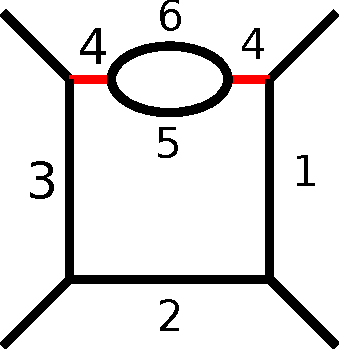
\includegraphics[width=\figureheight]{diagrams_from_4gluon/HexaBubbleThin}};
    \node at (0,1.5){(a) $\Gamma$, $\gleading$}; 
    \node at (1,2){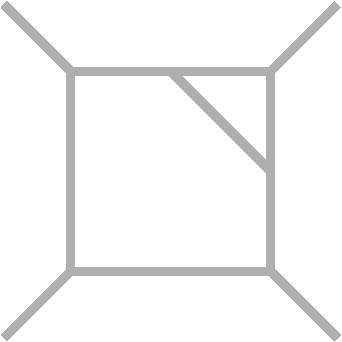
\includegraphics[width=\figureheight]{diagrams_from_4gluon/PentaTriangleThin}};
    \node at (2,2){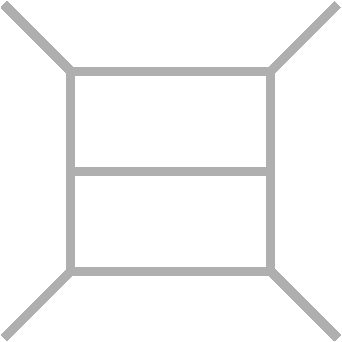
\includegraphics[width=\figureheight]{diagrams_from_4gluon/DoubleBoxThin}};
    \node at (3,2){\reflectbox{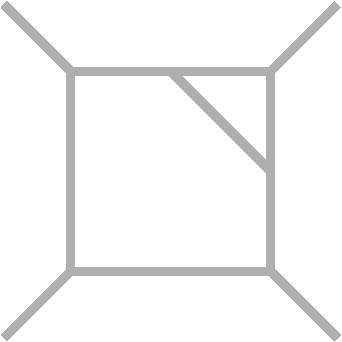
\includegraphics[width=\figureheight]{diagrams_from_4gluon/PentaTriangleThin}}};
        % Next-to-maximal
    \node at (0.5,1){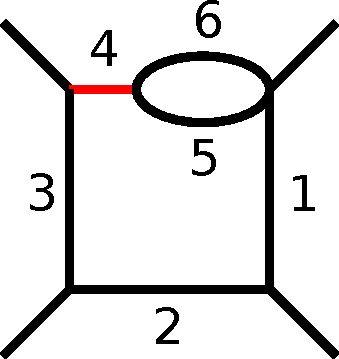
\includegraphics[width=\figureheight]{diagrams_from_4gluon/BubblePentagonSemiGenericThin}};
    \node at (0.5,0.5){(b) $\Gamma$, $\gamma_\Gamma^{(\hat{4})}$}; 
    \node at (1.5,1){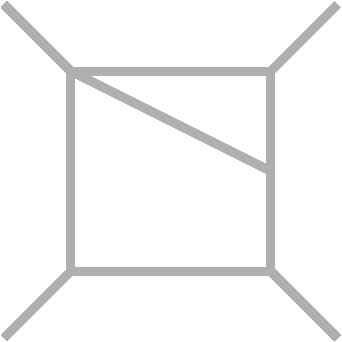
\includegraphics[width=\figureheight]{diagrams_from_4gluon/BoxTriangleThin}}; 
    \node at (2.5,1){\reflectbox{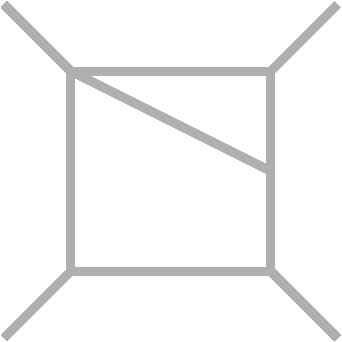
\includegraphics[width=\figureheight]{diagrams_from_4gluon/BoxTriangleThin}}};
        % Next-to-next-to-maximal
    \node at (1.5,0){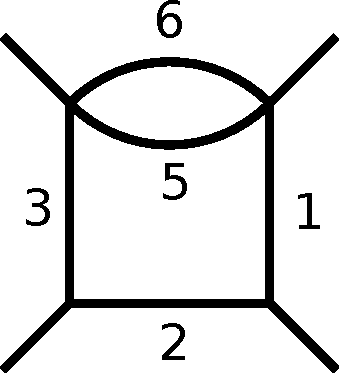
\includegraphics[width=\figureheight]{diagrams_from_4gluon/BubbleBoxGenericThin}};
    \node at (1.5,-0.5){(c) $\Gamma_{\hat{4}}$}; 
  \end{tikzpicture}
%
  \caption{The planar bubble-box hierarchy. The maximal diagrams are (a)-(d),
    next-to maximal are the (e)-(g) and at the bottom we find the bubble-box
    diagram (h).
    Based on the figure from \cite{Abreu:2017idw}. 
  }
  \label{fig:example_subleading_pole}
\end{figure}


}

\subsection{Evaluation of Cuts}
\label{sec:evluation_of_cuts}

\subsubsection{On-Shell Loop-Momenta}
\todo{In $D$ dimensions we don't have to worry about branches of solutions, and also loop momenta have to be real}


$D$-dimensional off-shell recursion,
the most practical and flexible way to compute them in $D$ dimensions is with off-shell recursions (see references e.g.\ in tails of 1001 gluons)

weyl and Dirac fermions,
tracking of representations?

states in appendix?

In the context of off-shell recursion it is more efficient to reverse
the decomposition of cut propagators into state sums, and treat them
as ``closed'' currents.

 
S-tree cuts (also reference Peraro's paper where this is explain as well)

Top-down and bottom-up.


\subsection{Dimensional Reconstruction}
 In $D$ and $D_s$ (dimensional reduction later)

see how \cref{chap:dshel} for discussion of what to do with $D_s$.

coefficients are $D$-dependent because of IBPs




\section{Discussion}
The two parts of our method are largely independent of each other and can be used separately if deemed beneficial.

Can be used to fit any integrand parametrization. For example one
can want to not have $D$-dependent coefficient, and fit to simple monomials.
Or one can eliminate transverse ISPs only, and do the IBP reduction later.
Or one can choose master/surface basis and do the full reduction in place.

Since the hardest problem is of IBP reduction it is beneficial to choose master/surface basis.

The factorization was not mandatory, lhs could be just evaluated and it could be anything.

